%for reference to this section
\section{Beschreibung}
\label{section:Beschreibung}

Generell sollte das Model selbsterklärend sein, der großteil der Beziehungen konnte direkt aus den Angaben ausgelesen werden. 
Es folgt eine kurze Beschreibung der wichtigsten Entitätsgruppen und Beziehungen:

\begin{description}
    \item[Zug, Wagon und Lokomotive] Der Zug und seine verknüpften Entitäten wurden aus der Angabe ausgelesen. 
    Klasse, Zugtyp, Wagontyp und Lokomotivtyp wurden als eigene Tabellen normiert. 
    Dies hat den Vorteil, dass diverse Preisinformationen ohne Redundanz verknüpft werden können.
    \item[Fahrplan und Strecke] Eine Strecke wurde als Summe von Streckenabschnitten (verknüpft mit einem Fahrplan) realisiert.
    Jeder Streckenabschnitt hat einen Abfahrtsbahnsteig (mit Uhrzeit), und einen Ankunftsbahnsteig (ebenfalls mit Uhrzeit). 
    Der Start eines Fahrplans ist der Abfahrtsbahnsteig jenes Streckenabschnitts, der die geringste Uhrzeit hat, 
    und das Ende eines Fahrplans ist, komplementär, der Ankunftsbahnsteig jenes Streckenabschnitts, der die höchste Uhrzeit hat.
    \item[Bahnhof] Der Bahnhof ist selbsterklärend: Jeder Bahnhof besitzt mindestens einen Bahnsteig. 
    Der Ort eines Bahnhofs wurde als eigene Tabelle normiert, da auch eine Kundin einem Ort zugeteilt ist.
    \item[Ticket] Die Tickets wurden als ein hierarchisches Vererbungsmodell realisiert. Jedes Ticket hat eine Nummer und ein Gültigkeitsdatum.
    Einem Dauerticket ist dabei eine Kundin zugeordnet. Zusätzlich hat das Dauerticket einen Dauertyp (Jahr, Monat, Woche), 
    der zusätzlich zum Gültigkeitsdatum (``Startdatum'') das Ende des Dauertickets bestimmt.
    Einer anonymen Einzelfahrt sind zwei Bahnsteige zugeordnet (``von'', ``bis'').
    Hat der Kunde eine Sitzplatzreservierung erstanden, so ist auch ein eindeutiger Sitzplatz dem Ticket zugewiesen.
    Die Beziehung zwischen Sitzplatz und Einzelfahrt mit Reservierung ist eine 1:N, da ein Sitzplatz zu verschiedenen Zeiten 
    von verschiedenen Kunden reserviert werden kann.
    \item[Preis] Die verschiedenen Preise (``Preis je Haltestelle'', ``Dauerticketpreis'', ``Einzelticketpreis'' und ``Reservierungsaufschlag'') 
    sind mit den relevanten Tabellen verknüpft. Zusätzlich hat jeder Preis ein Gültigkeitsdatum (``von'', ``bis''). 
    Damit können Periserhöhungen schon im Vorfeld in das Datenmodell eingetragen werden, und haben erst ab einem bestimmten Tag eine Auswirkung auf die Ticketpreise.

\end{description}
\begin{figure}[h]
    \caption{Logisches Modell}
    \centering
    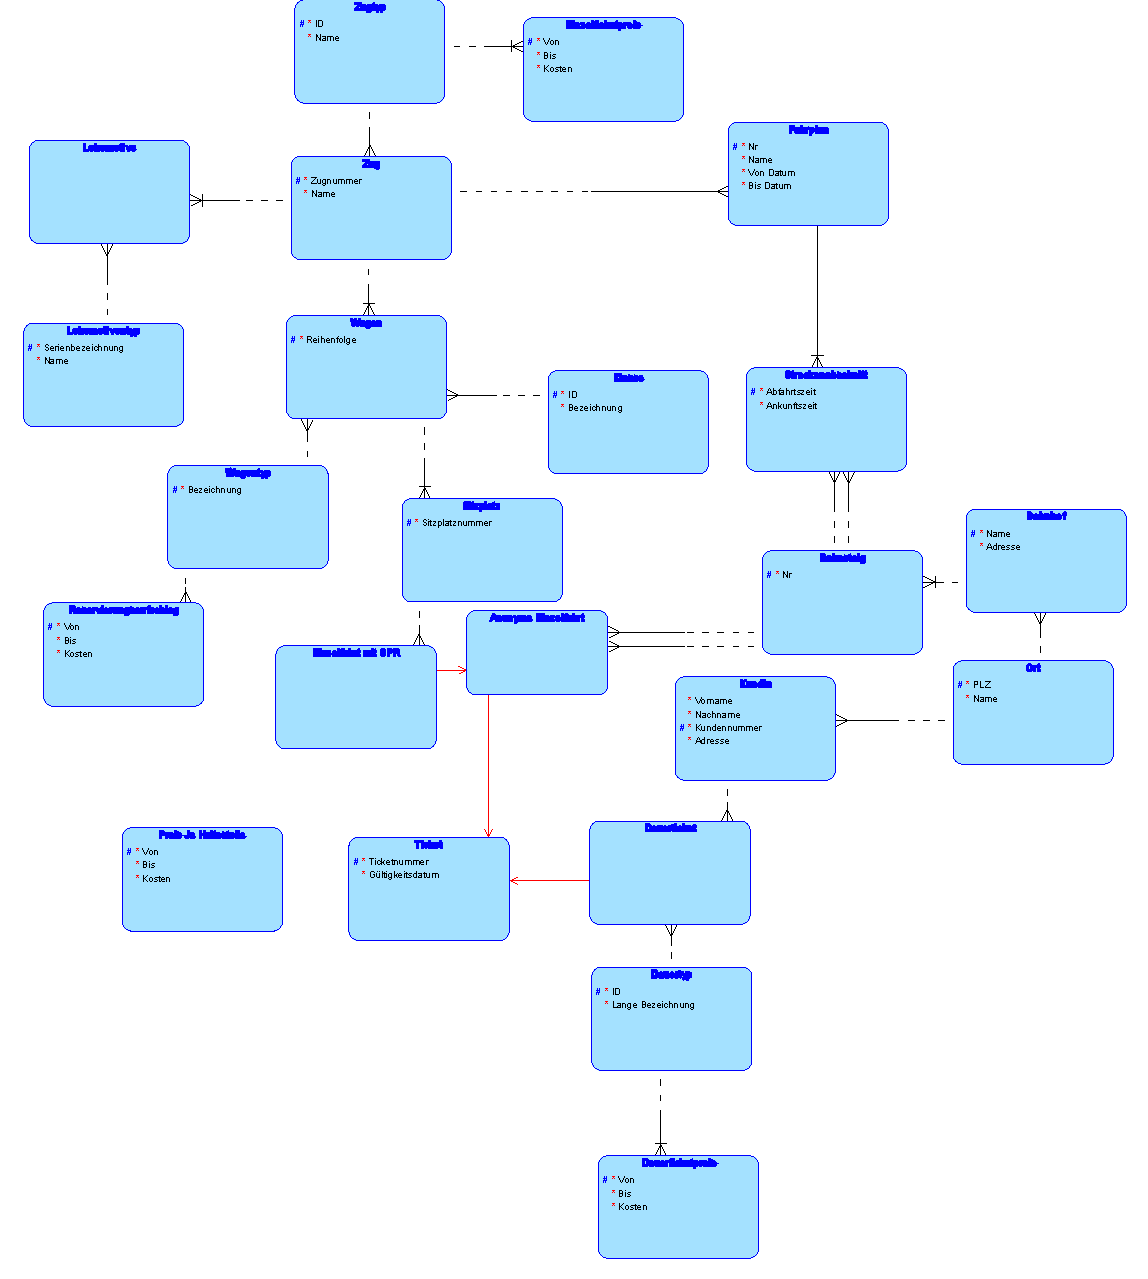
\includegraphics[width=1\textwidth]{logical}
    \end{figure}
\section{Diagramm}
\label{section:Diagramm}
